% II2202 Quantitative exercise. Compile with `make` in this folder (LuaLaTeX in Docker).
% Every data value is a macro \V{key} defined in numbers.tex, which make_numbers.py
% generates from results/stats/*.csv. Do not type data values by hand.
\documentclass[11pt,a4paper]{article}
\usepackage{fontspec}
\setmainfont{Source Sans 3}
\setsansfont{Source Sans 3}
\setmonofont{Latin Modern Mono}[Scale=0.95]
\usepackage[english]{babel}
\usepackage[margin=2.54cm,headsep=14pt]{geometry}
\usepackage{fancyhdr}
\usepackage{lastpage}
\usepackage{graphicx}
\usepackage{booktabs}
\usepackage{tabularx}
\usepackage{array}
\usepackage{enumitem}
\usepackage{amsmath}
\usepackage{caption}
\usepackage{subcaption}
\usepackage{titlesec}
\usepackage{microtype}
\usepackage[hidelinks]{hyperref}
\usepackage{xcolor}

% Generated by make_numbers.py from results/stats/*.csv. Do not edit.
\makeatletter
\newcommand{\V}[1]{\ifcsname v@#1\endcsname\csname v@#1\endcsname\else\errmessage{Undefined value #1}\fi}
\expandafter\def\csname v@be.sf1\endcsname{$-$21.6}
\expandafter\def\csname v@be.sf10\endcsname{$-$20.0}
\expandafter\def\csname v@headline.boot_median_halfwidth_n3_pct\endcsname{7.1}
\expandafter\def\csname v@headline.ch_client_overhead_median_ms\endcsname{0.8}
\expandafter\def\csname v@headline.cold_ch_faster_queries_sf10\endcsname{Q6, Q3, Q13}
\expandafter\def\csname v@headline.cold_ch_faster_ratio_max\endcsname{0.93}
\expandafter\def\csname v@headline.cold_ch_faster_ratio_min\endcsname{0.87}
\expandafter\def\csname v@headline.cold_flip_queries_sf1\endcsname{Q13}
\expandafter\def\csname v@headline.cold_flip_queries_sf10\endcsname{Q6, Q3, Q18}
\expandafter\def\csname v@headline.cold_over_warm_max\endcsname{5.2}
\expandafter\def\csname v@headline.cold_over_warm_median\endcsname{2.3}
\expandafter\def\csname v@headline.cold_over_warm_min\endcsname{1.3}
\expandafter\def\csname v@headline.cv_max_pct\endcsname{23}
\expandafter\def\csname v@headline.disk_ratio_sf1\endcsname{1.57}
\expandafter\def\csname v@headline.disk_ratio_sf10\endcsname{1.69}
\expandafter\def\csname v@headline.duck_faster_ratio_max\endcsname{4.01}
\expandafter\def\csname v@headline.duck_faster_ratio_min\endcsname{1.26}
\expandafter\def\csname v@headline.engine_peak_max_gib_clickhouse_sf10\endcsname{1.69}
\expandafter\def\csname v@headline.engine_peak_max_gib_duckdb_sf10\endcsname{1.44}
\expandafter\def\csname v@headline.full_study_query_runs\endcsname{1344}
\expandafter\def\csname v@headline.idle_gib_clickhouse_sf1\endcsname{1.28}
\expandafter\def\csname v@headline.idle_gib_duckdb_sf1\endcsname{0.08}
\expandafter\def\csname v@headline.load_ratio_sf1\endcsname{3.0}
\expandafter\def\csname v@headline.load_ratio_sf10\endcsname{3.3}
\expandafter\def\csname v@headline.mw_min_p_5v5\endcsname{0.008}
\expandafter\def\csname v@headline.n_combos\endcsname{32}
\expandafter\def\csname v@headline.n_comparisons\endcsname{16}
\expandafter\def\csname v@headline.n_cv_below_10\endcsname{19}
\expandafter\def\csname v@headline.n_duck_faster\endcsname{13}
\expandafter\def\csname v@headline.n_min_n_not_reached\endcsname{5}
\expandafter\def\csname v@headline.n_runs\endcsname{672}
\expandafter\def\csname v@headline.n_runs_spilled\endcsname{0}
\expandafter\def\csname v@headline.n_shapiro_reject\endcsname{26}
\expandafter\def\csname v@headline.n_significant\endcsname{15}
\expandafter\def\csname v@headline.n_slope_ci_above_1\endcsname{2}
\expandafter\def\csname v@headline.n_slope_ci_below_1\endcsname{9}
\expandafter\def\csname v@headline.order_max_halfwidth_n20_pct\endcsname{9.7}
\expandafter\def\csname v@headline.order_median_halfwidth_n20_pct\endcsname{3.2}
\expandafter\def\csname v@headline.order_share_below_5pct_n10_pct\endcsname{28}
\expandafter\def\csname v@headline.order_share_below_5pct_n15_pct\endcsname{62}
\expandafter\def\csname v@headline.order_share_below_5pct_n20_pct\endcsname{84}
\expandafter\def\csname v@headline.peak_max_gib\endcsname{4.89}
\expandafter\def\csname v@headline.peak_ratio_max_sf1\endcsname{7.0}
\expandafter\def\csname v@headline.peak_ratio_max_sf10\endcsname{2.8}
\expandafter\def\csname v@headline.peak_ratio_min_sf1\endcsname{4.6}
\expandafter\def\csname v@headline.peak_ratio_min_sf10\endcsname{1.6}
\expandafter\def\csname v@headline.pilot_load_minutes\endcsname{7}
\expandafter\def\csname v@headline.pilot_query_minutes\endcsname{6}
\expandafter\def\csname v@headline.ratio_min_q1_q21\endcsname{2.97}
\expandafter\def\csname v@headline.slope_max\endcsname{1.08}
\expandafter\def\csname v@headline.slope_median\endcsname{0.98}
\expandafter\def\csname v@headline.slope_min\endcsname{0.93}
\expandafter\def\csname v@load.anon_max_sf10\endcsname{3.07}
\expandafter\def\csname v@memory.max_gap_pct\endcsname{2.0}
\expandafter\def\csname v@memory.max_interval_ms\endcsname{4.8}
\expandafter\def\csname v@memory.median_interval_ms\endcsname{3.5}
\expandafter\def\csname v@memory.share_below_1pct\endcsname{99.7}
\expandafter\def\csname v@pca.pc1_pct\endcsname{69}
\expandafter\def\csname v@pca.pc2_pct\endcsname{17}
\expandafter\def\csname v@q13sf1.ratio\endcsname{0.89}
\expandafter\def\csname v@q13sf10.ratio\endcsname{0.92}
\expandafter\def\csname v@q18sf10.p_holm\endcsname{0.29}
\expandafter\def\csname v@q18sf10.ratio\endcsname{0.98}
\expandafter\def\csname v@q18sf10.ratio_hi\endcsname{1.02}
\expandafter\def\csname v@q18sf10.ratio_lo\endcsname{0.93}
\expandafter\def\csname v@setup.ch_max_threads\endcsname{4}
\expandafter\def\csname v@setup.clickhouse_version\endcsname{26.8.36.3}
\expandafter\def\csname v@setup.cpu_model\endcsname{Apple M1 Pro}
\expandafter\def\csname v@setup.docker_version\endcsname{29.0.1}
\expandafter\def\csname v@setup.docker_vm_mem_mib\endcsname{10240}
\expandafter\def\csname v@setup.duck_threads\endcsname{4}
\expandafter\def\csname v@setup.duckdb_version\endcsname{2.0.0}
\expandafter\def\csname v@setup.host_cores\endcsname{8}
\expandafter\def\csname v@setup.host_mem_gib\endcsname{16}
\expandafter\def\csname v@setup.kernel\endcsname{6.12.54-linuxkit}
\expandafter\def\csname v@setup.sf10_parquet_gb\endcsname{3.42}
\expandafter\def\csname v@setup.sf10_total_rows\endcsname{86,586,082}
\expandafter\def\csname v@setup.sf1_parquet_gb\endcsname{0.32}
\expandafter\def\csname v@setup.sf1_total_rows\endcsname{8,661,245}
\expandafter\def\csname v@slope.ch21\endcsname{1.08}
\makeatother


\newcommand{\reportdate}{November 5, 2026}
\pagestyle{fancy}
\fancyhf{}
\renewcommand{\headrulewidth}{0pt}
\fancyhead[L]{\small II2202, Autumn 2026, Period 2}
\fancyhead[C]{\small Quantitative exercise}
\fancyhead[R]{\small \reportdate}
\fancyfoot[R]{\small \thepage\ (\pageref*{LastPage})}
\fancypagestyle{plain}{\fancyhf{}\fancyhead[L]{\small II2202, Autumn 2026, Period 2}%
  \fancyhead[C]{\small Quantitative exercise}\fancyhead[R]{\small \reportdate}%
  \fancyfoot[R]{\small \thepage\ (\pageref*{LastPage})}}

\titleformat{\section}{\Large\bfseries}{\thesection}{1em}{}
\titleformat{\subsection}{\large\bfseries}{\thesubsection}{1em}{}
\titlespacing*{\section}{0pt}{10pt}{5pt}
\titlespacing*{\subsection}{0pt}{9pt}{4pt}
\setlength{\parindent}{0pt}
\setlength{\parskip}{4.5pt}
\captionsetup{font=small,labelfont=bf,skip=4pt}
\setlist{itemsep=1pt,topsep=2pt}
\renewcommand{\arraystretch}{1.08}
\newcolumntype{L}{>{\raggedright\arraybackslash}X}
\newcommand{\Q}[1]{Q#1}
\newcommand{\CH}{ClickHouse}
\newcommand{\DK}{DuckDB}

\begin{document}

{\LARGE\bfseries Quantitative exercise: a pilot benchmark of ClickHouse and DuckDB under an 8\,GiB, four-core budget\par}
\vspace{14pt}
{\Large\bfseries Authors\par}
\vspace{6pt}
Weizhuo Sun <weizhuo@kth.se>

Weiyin Fang <weiyinf@kth.se>

\section{Introduction}

Our project compares a server-based column store (\CH) with an embedded engine (\DK) for gigabyte-scale analytics under one fixed budget of 8\,GiB memory and four cores.
It asks about query latency (RQ1), memory and disk footprint (RQ2), and load time and the number of query runs needed to pay it back (RQ3).
For this exercise we built the measurement set-up and ran a small pilot of the planned experiment; all data below come from it.
Its main use is to decide which data the full study must collect, and how much.

\section{Dataset (a)}

\textbf{Workload.} We generated TPC-H data~\cite{tpch} at scale factors 1 and 10 (SF1, SF10) with the \texttt{dbgen} function of \DK's \texttt{tpch} extension, and exported each of the eight tables to Parquet.
SF1 has \V{setup.sf1_total_rows} rows (\V{setup.sf1_parquet_gb}\,GB of Parquet) and SF10 has \V{setup.sf10_total_rows} rows (\V{setup.sf10_parquet_gb}\,GB).
The row counts of all tables match the TPC-H specification.
Both engines load the same files.
We use the eight queries of our research plan, grouped by their main access pattern: scan (\Q1, \Q6), join (\Q5, \Q9, \Q21) and aggregation (\Q3, \Q13, \Q18).
The query texts are the TPC-H queries with the default substitution parameters, taken from \DK's \texttt{tpch} extension.
\CH\ runs all of them unchanged except one: \Q13 needs \texttt{SETTINGS join\_use\_nulls = 1}.
Without it \CH\ fills unmatched rows of the outer join with 0 instead of NULL, and the result is wrong.

\textbf{Systems and set-up.} Table~\ref{tab:setup} lists the configuration.
Each engine runs in its own Docker container with \texttt{--memory=8g --memory-swap=8g --cpus=4} on the same four virtual CPUs.
\DK\ is embedded, so its container runs a small Python process that holds the connection, as an application would; a driver container on the other four virtual CPUs runs the experiment.
The host is a laptop (\V{setup.cpu_model}, \V{setup.host_cores} cores, \V{setup.host_mem_gib}\,GiB) running Docker Desktop \V{setup.docker_version}, whose Linux virtual machine has \V{setup.docker_vm_mem_mib}\,MiB of memory and kernel \V{setup.kernel}.

\begin{table}[ht]
\centering\small
\caption{Fixed configuration. Memory settings were chosen so that each engine stays below the container limit.}
\label{tab:setup}
\begin{tabularx}{\textwidth}{@{}lLL@{}}
\toprule
 & \CH & \DK \\
\midrule
Version & \V{setup.clickhouse_version} (LTS), official image & \V{setup.duckdb_version}, Python API in \texttt{python:3.12-slim} \\
Container & 8\,GiB memory, no swap, 4 CPUs & same \\
Engine memory limit & \texttt{max\_server\_memory\_usage} = 7\,GiB & \texttt{memory\_limit} = 7\,GiB \\
Threads & \texttt{max\_threads} = \V{setup.ch_max_threads} & \texttt{threads} = \V{setup.duck_threads} \\
Spilling & GROUP BY, ORDER BY above 3\,GiB; joins in memory & to \texttt{/tmp/duck\_spill} \\
Storage, caches & MergeTree on TPC-H primary key; query (condition) cache off & one \texttt{.duckdb} file; no result cache \\
\bottomrule
\end{tabularx}
\end{table}

\textbf{Procedure.} For each engine and SF we loaded the data three times.
Each load starts from a restarted engine and an emptied operating-system page cache, imports all tables and is timed.
For \CH\ the background merges are then forced with \texttt{OPTIMIZE~...~FINAL} and timed separately; for \DK\ the \texttt{CHECKPOINT} is timed.
For each engine, SF and query we then restarted the engine, emptied the page cache and ran the query once (\emph{cold}), followed by 20 runs in a row (\emph{warm}).
This gives \V{headline.n_runs} query runs and 12 loads.
Query order was shuffled with a fixed seed.
Before any timing, a correctness check compared every result at SF1 with the TPC-H reference answers, and compared the two engines with each other at both SFs.
All checks passed, and every timed run returned the verified result.

\section{Variables and expected properties (b)}

Table~\ref{tab:vars} lists the variables.
We wrote down the expected properties below before the analysis, and we did not change them afterwards.

\begin{table}[ht]
\centering\small
\caption{Independent and dependent variables.}
\label{tab:vars}
\begin{tabularx}{\textwidth}{@{}llL@{}}
\toprule
Variable & Type & Values or unit \\
\midrule
Engine & independent, categorical & \CH, \DK \\
Scale factor (SF) & independent, ordinal & 1, 10 \\
Query class & independent, categorical & scan, join, aggregation (query as blocking factor) \\
Phase & independent, categorical & cold (first run after restart), warm \\
Latency & dependent, continuous & ms, wall-clock per query run \\
Peak memory & dependent, continuous & bytes, maximum of the container's memory during a run \\
Load time & dependent, continuous & s, import (plus merge or checkpoint) of all tables \\
Disk footprint & dependent, continuous & bytes on disk after loading \\
\bottomrule
\end{tabularx}
\end{table}

\begin{enumerate}[label=E\arabic*.,leftmargin=2.2em,itemsep=0pt]
\item Latency is positive and right-skewed with a long tail.
\item Cold runs are clearly slower than warm runs.
\item Warm runs vary little: coefficient of variation (CV) below 10\,\%.
\item Latency grows roughly linearly with SF, so the slope in log--log coordinates is about 1.
\item \CH\ is faster on join and aggregation queries.
\item \DK\ loads faster and uses less memory when idle.
\item Peak memory grows with SF but stays below the 7\,GiB engine limit; above it, the engines spill to disk instead of failing.
\item \CH's compressed disk footprint is smaller than \DK's file, or similar.
\end{enumerate}

\section{Data analysis (c)}

\textbf{Preprocessing.} The driver writes one CSV row per run. A script checks that all \V{headline.n_runs} runs and 12 loads are present, every result is correct, every latency is positive and no peak exceeds 8\,GiB. No run failed and no row was removed.

\textbf{Measurement of memory.} \CH\ is a server while \DK\ shares a process with its host, so there is no common process boundary; we measure both at the container.
The driver reads the container's \texttt{memory.current} every 2\,ms during each run (actual median interval \V{memory.median_interval_ms}\,ms, maximum \V{memory.max_interval_ms}\,ms) and takes the maximum.
As a check, it also resets and reads the kernel's exact high-water mark (\texttt{memory.peak}).
The sampled maximum is within 1\,\% of it in \V{memory.share_below_1pct}\,\% of the runs and never more than \V{memory.max_gap_pct}\,\% below it.
This container-level number includes the page cache of files the engine has read or written, so we also record the anonymous (heap) memory, and each engine's own number: the \texttt{memory\_usage} in \CH's query log, and the resident set size of the \DK\ process.

\textbf{Exploratory analysis.} We plotted every run (Figure~\ref{fig:latency}), tested normality with the Shapiro--Wilk test, computed the CV and checked each expectation against the data.

\textbf{Statistical methods.} Because latency is skewed (Section~\ref{sec:results}), we use medians and nonparametric methods~\cite{hoefler}.
\begin{enumerate}[leftmargin=1.5em]
\item For each engine, SF and query: median of the 20 warm runs with a 95\,\% percentile-bootstrap confidence interval (CI; 10\,000 resamples, fixed seed).
\item Engine comparison per SF and query: ratio of medians (\CH/\DK) with a bootstrap CI, two-sided Mann--Whitney U test with Holm correction over the eight queries of each SF, and Cliff's $\delta$ as effect size~\cite{romano}.
\item Scaling model: for each engine and query we fit $\log t = a + b \log \mathrm{SF}$.
With only two SF values the line passes exactly through both medians, so it has no residuals and cannot be tested; the CI of $b$ only reflects run-to-run noise.
\item Break-even (RQ3): the total cost of loading once and running the query set $n$ times is $T(n) = L + n\,q$, where $L$ is the median load time (import plus merge or checkpoint) and $q$ the sum of the eight median warm latencies.
Two lines cross at $n^* = (L_A - L_B)/(q_B - q_A)$; if $n^* \le 0$, one engine is cheaper for every $n$.
\item How much data is needed: we recomputed the 95\,\% CI of the median from only the first $n$ warm runs ($n$ = 3, 5, 6, 10, 15, 20) and looked for the smallest $n$ with a relative half-width below 5\,\%.
We use the exact distribution-free CI based on order statistics~\cite{leboudec}, which does not exist for $n < 6$, because the bootstrap CI is far too narrow for tiny samples: at $n = 3$ it is the range of the three values and contains the true median only 75\,\% of the time (confirmed in a simulation test).
\item Searching for a model (PCA): we built a matrix with one row per query and eight columns (log median latency and log median peak memory for each engine and SF), standardised the columns and ran a principal component analysis, to see whether the queries group by our three classes.
\end{enumerate}

\section{Results (d)}
\label{sec:results}

\textbf{Latency (RQ1).} Figure~\ref{fig:latency} shows all warm runs and the cold run.
Contrary to E5, \DK\ was faster in \V{headline.n_duck_faster} of the \V{headline.n_comparisons} comparisons, by a factor of \V{headline.duck_faster_ratio_min} to \V{headline.duck_faster_ratio_max} (Table~\ref{tab:latency}).
\CH\ was faster only on \Q13 at both SFs (ratio \V{q13sf1.ratio} and \V{q13sf10.ratio}) and on \Q18 at SF10, where the difference (ratio \V{q18sf10.ratio}, CI \V{q18sf10.ratio_lo}--\V{q18sf10.ratio_hi}) is not significant (Holm-adjusted $p = \V{q18sf10.p_holm}$).
The other \V{headline.n_significant} differences are significant (adjusted $p \le \V{headline.max_p_holm_significant}$) with a large effect size.
The gap depends more on the query than on its class: it is largest for \Q1 and \Q21 (ratio at least \V{headline.ratio_min_q1_q21}) and smallest for \Q9, \Q13 and \Q18.
With one cold run per query the cold differences cannot be tested.
At SF1 the cold runs ranked the engines as the warm runs did, but at SF10 \CH's cold run was faster for \V{headline.n_cold_ch_faster_sf10} queries (\Q3, \Q6, \Q13; ratio \V{headline.cold_ch_faster_ratio_min}--\V{headline.cold_ch_faster_ratio_max}).
\CH's HTTP interface adds little: the client latency exceeds the server's own time by a median of \V{headline.ch_client_overhead_median_ms}\,ms.

\begin{figure}[ht]
\centering
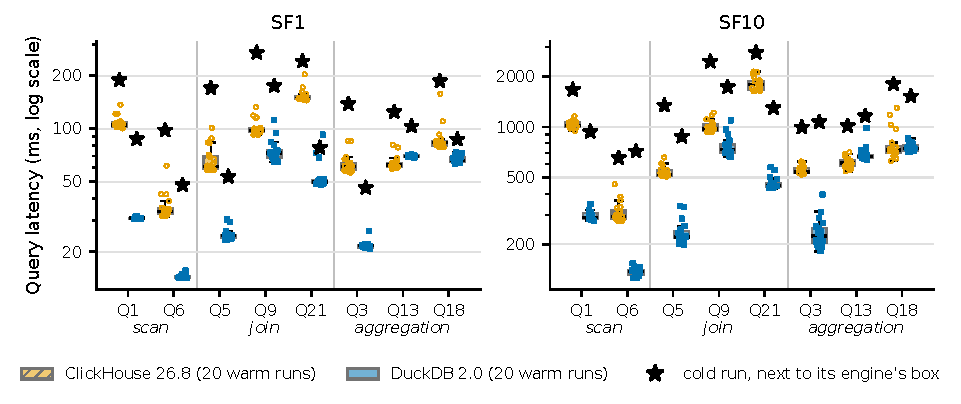
\includegraphics[width=\textwidth]{../figures/F1_latency.pdf}
\caption{Warm latency per query (box: quartiles and median; points: the 20 runs) and the cold run (star) for each engine. Log scale; note the different axes for SF1 and SF10.}
\label{fig:latency}
\end{figure}

\begin{table}[ht]
\centering\footnotesize
\setlength{\tabcolsep}{4.5pt}
\caption{Warm latency per query: median of 20 runs [95\,\% bootstrap CI] in ms, ratio of medians \CH/\DK\ [95\,\% CI], Holm-adjusted $p$ of the Mann--Whitney test and Cliff's $\delta$ (negative: \CH\ faster).}
\label{tab:latency}
\begin{tabular}{@{}rlllllrr@{}}
\toprule
SF & Query & Class & \CH\ (ms) & \DK\ (ms) & Ratio & $p_\mathrm{Holm}$ & $\delta$ \\
\midrule
1 & Q1 & scan & 105 [103, 107] & 31.0 [30.8, 31.1] & 3.39 [3.32, 3.47] & $<$0.001 & 1.00 \\
1 & Q6 & scan & 33.6 [32.8, 35.0] & 14.3 [14.2, 14.4] & 2.35 [2.29, 2.45] & $<$0.001 & 1.00 \\
1 & Q5 & join & 61.1 [59.6, 68.2] & 24.6 [24.1, 24.8] & 2.49 [2.42, 2.78] & $<$0.001 & 1.00 \\
1 & Q9 & join & 97.3 [96.1, 100] & 72.7 [68.7, 74.4] & 1.34 [1.31, 1.43] & $<$0.001 & 0.90 \\
1 & Q21 & join & 148 [147, 151] & 49.7 [49.0, 50.9] & 2.97 [2.90, 3.05] & $<$0.001 & 1.00 \\
1 & Q3 & aggregation & 60.9 [58.1, 62.9] & 21.6 [21.3, 21.8] & 2.82 [2.68, 2.93] & $<$0.001 & 1.00 \\
1 & Q13 & aggregation & 62.1 [60.7, 63.4] & 69.6 [69.4, 69.9] & 0.89 [0.87, 0.91] & $<$0.001 & $-$0.80 \\
1 & Q18 & aggregation & 83.0 [80.7, 83.7] & 65.6 [64.9, 68.4] & 1.26 [1.20, 1.28] & $<$0.001 & 1.00 \\
\midrule
10 & Q1 & scan & 1022 [1005, 1051] & 290 [283, 303] & 3.52 [3.35, 3.65] & $<$0.001 & 1.00 \\
10 & Q6 & scan & 292 [285, 313] & 138 [134, 139] & 2.12 [2.06, 2.29] & $<$0.001 & 1.00 \\
10 & Q5 & join & 523 [516, 544] & 221 [219, 236] & 2.37 [2.21, 2.46] & $<$0.001 & 1.00 \\
10 & Q9 & join & 973 [957, 1020] & 736 [706, 778] & 1.32 [1.25, 1.42] & $<$0.001 & 0.88 \\
10 & Q21 & join & 1795 [1690, 1853] & 448 [441, 459] & 4.01 [3.72, 4.13] & $<$0.001 & 1.00 \\
10 & Q3 & aggregation & 539 [533, 565] & 225 [206, 244] & 2.40 [2.20, 2.68] & $<$0.001 & 1.00 \\
10 & Q13 & aggregation & 610 [587, 627] & 667 [655, 677] & 0.92 [0.88, 0.95] & $<$0.001 & $-$0.78 \\
10 & Q18 & aggregation & 730 [706, 751] & 741 [722, 768] & 0.98 [0.93, 1.02] & 0.29 & $-$0.20 \\
\bottomrule
\end{tabular}
\end{table}


\textbf{Distribution and noise (E1--E3).} All \V{headline.n_combos} warm distributions are right-skewed, and the Shapiro--Wilk test rejects normality for \V{headline.n_shapiro_reject} of them, so medians are the right summary (E1 holds).
The cold run took \V{headline.cold_over_warm_min} to \V{headline.cold_over_warm_max} times the warm median (median \V{headline.cold_over_warm_median}; E2 holds).
E3 holds only partly: the CV was below 10\,\% in \V{headline.n_cv_below_10} of \V{headline.n_combos} combinations and reached \V{headline.cv_max_pct}\,\%.
Most of the variation comes from a few slow outliers (Figure~\ref{fig:latency}), not from a wide spread.

\textbf{Scaling (E4).} Figure~\ref{fig:scaling} shows that the lines of all queries run nearly parallel to the slope-1 reference.
The fitted slopes lie between \V{headline.slope_min} and \V{headline.slope_max} (median \V{headline.slope_median}), so latency grows about linearly with data size and E4 holds.
The CI excludes 1 for \V{headline.n_slope_ci_below_1} slopes below 1 and \V{headline.n_slope_ci_above_1} above 1 (\CH\ \Q21: \V{slope.ch21}), but with two SF points we cannot tell whether this is a real deviation from linearity or a fixed per-query cost.

\begin{figure}[ht]
\centering
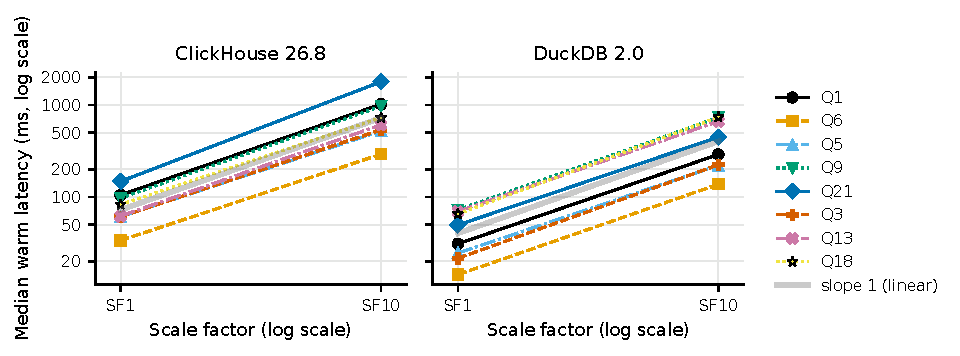
\includegraphics[width=0.81\textwidth]{../figures/F2_scaling.pdf}
\caption{Median warm latency against scale factor (both axes logarithmic). The thick grey line has slope 1 (latency proportional to SF).}
\label{fig:scaling}
\end{figure}

\textbf{Memory (RQ2, E6--E7).} Figure~\ref{fig:memory} shows the peak container memory.
\DK\ needed much less: \CH's median peak was \V{headline.peak_ratio_min_sf1}--\V{headline.peak_ratio_max_sf1} times \DK's at SF1 and \V{headline.peak_ratio_min_sf10}--\V{headline.peak_ratio_max_sf10} times at SF10.
A large part of this is the idle footprint: right after a restart the \CH\ container already used \V{headline.idle_gib_clickhouse_sf1}\,GiB, against \V{headline.idle_gib_duckdb_sf1}\,GiB for \DK\ (SF1; E6 holds for memory).
Peak memory grew with SF for every engine and query.
The highest peak of any run was \V{headline.peak_max_gib}\,GiB (\CH, \Q18, SF10), well below the 7\,GiB limit, so no run spilled to disk and none failed.
E7 therefore holds, but its second half (spilling instead of failing) was not tested.
The two engines' own numbers are smaller than the container peaks, because the container also counts page cache and, for \CH, the idle server: the largest median was \V{headline.engine_peak_max_gib_clickhouse_sf10}\,GiB in \CH's query log and \V{headline.engine_peak_max_gib_duckdb_sf10}\,GiB of \DK\ process memory (SF10).

\begin{figure}[ht]
\centering
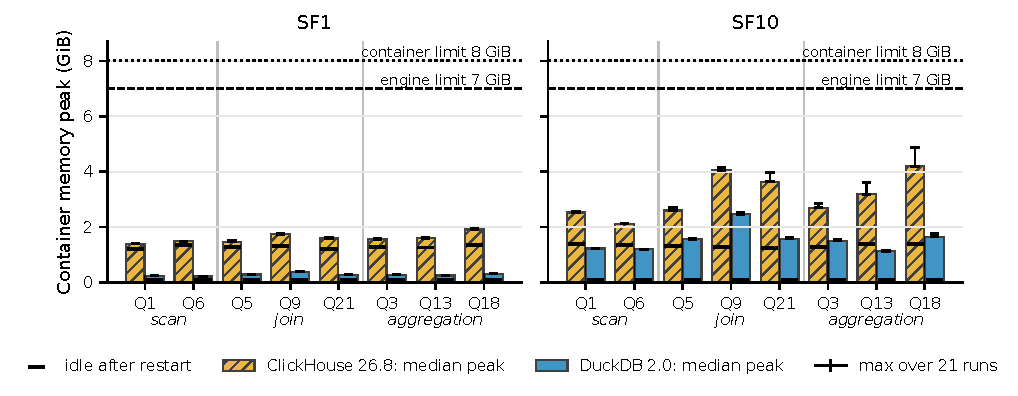
\includegraphics[width=\textwidth]{../figures/F3_memory.pdf}
\caption{Peak container memory during warm runs (bar: median; whisker: maximum over all 21 runs) and the container's memory right after restart (black dash). Dashed and dotted lines: engine and container limits.}
\label{fig:memory}
\end{figure}

\textbf{Load time and disk (RQ2--RQ3, E6, E8).} Table~\ref{tab:load} lists the loads.
\DK\ loaded \V{headline.load_ratio_sf1} times faster at SF1 and \V{headline.load_ratio_sf10} times faster at SF10 (E6 holds).
For \CH, the forced merge takes almost as long as the import itself, while \DK's final checkpoint at SF10 takes only milliseconds because \DK\ already writes checkpoints during the import.
E8 does not hold: \CH's tables took \V{headline.disk_ratio_sf1} (SF1) and \V{headline.disk_ratio_sf10} (SF10) times the space of the \DK\ file, and more than the Parquet input, while the \DK\ file was smaller than the Parquet input.
A likely reason is that \CH\ by default compresses with LZ4, which favours speed over size, but we did not test this.
During the SF10 loads the container memory of both engines reached the 8\,GiB limit.
This is page cache of the files being written, which the kernel reclaims; the anonymous memory stayed at or below \V{load.anon_max_sf10}\,GiB and no load failed.

\begin{table}[ht]
\centering\footnotesize
\caption{Loads (3 per engine and SF). Each column is the median of its own three values, so Total need not equal Import + Merge/ckpt: import time (min--max), merge (\CH) or checkpoint (\DK) time, total; disk footprint and its ratio to the Parquet input (computed from unrounded sizes); peak container / anonymous memory during the load (maximum); container memory right after restart (median over the cold runs). GB = $10^9$ bytes, GiB = $2^{30}$ bytes.}
\label{tab:load}
\setlength{\tabcolsep}{4pt}
\begin{tabular}{@{}lrrrrrrrr@{}}
\toprule
Engine & SF & Import (s) & Merge/ckpt (s) & Total (s) & Disk (GB) & Disk/Parquet & Load peak (GiB) & Idle (GiB) \\
\midrule
\CH & 1 & 5.2 (5.0--6.5) & 4.6 & 9.8 & 0.47 & 1.44 & 3.83 / 2.50 & 1.28 \\
\DK & 1 & 3.1 (2.8--3.3) & 0.20 & 3.2 & 0.30 & 0.92 & 1.29 / 0.68 & 0.08 \\
\CH & 10 & 47.5 (44.4--47.7) & 40.5 & 87.1 & 4.73 & 1.38 & 8.00 / 2.96 & 1.33 \\
\DK & 10 & 26.7 (25.8--27.5) & 0.003 & 26.7 & 2.80 & 0.82 & 8.00 / 3.07 & 0.09 \\
\bottomrule
\end{tabular}
\end{table}


\textbf{Break-even (RQ3).} \DK\ both loads and queries faster, so the cost lines never cross for $n > 0$ (Figure~\ref{fig:breakeven}).
The formula gives $n^*$ = \V{be.sf1} at SF1 and \V{be.sf10} at SF10, and none of the bootstrap resamples gave a positive $n^*$.
In this pilot \DK\ is cheaper for any number of runs.

\begin{figure}[ht]
\centering
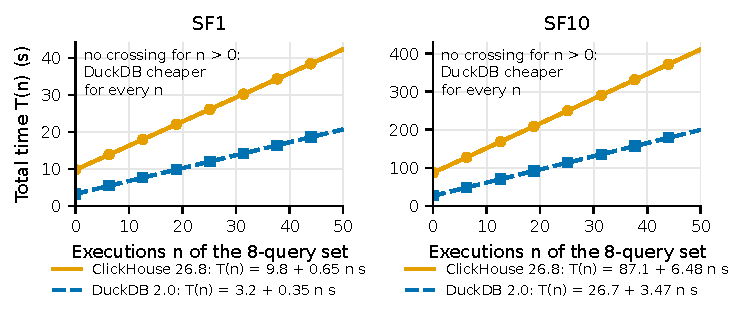
\includegraphics[width=0.8\textwidth]{../figures/F4_breakeven.pdf}
\caption{Total cost $T(n)$ of loading once and running the 8-query set $n$ times. Intercept: median load time; slope: sum of median warm latencies.}
\label{fig:breakeven}
\end{figure}

\textbf{How many runs are needed.} Figure~\ref{fig:reps} shows how the CI of the median narrows as more warm runs are used.
With the exact CI, a half-width below 5\,\% was reached for \V{headline.order_share_below_5pct_n10_pct}\,\% of the combinations with 10 runs, \V{headline.order_share_below_5pct_n15_pct}\,\% with 15 runs and \V{headline.order_share_below_5pct_n20_pct}\,\% with 20 runs.
With 20 runs the median half-width was \V{headline.order_median_halfwidth_n20_pct}\,\% and the largest \V{headline.order_max_halfwidth_n20_pct}\,\%.
For \V{headline.n_min_n_not_reached} combinations even 20 runs were not enough.
The bootstrap line shows why small samples are misleading: at $n = 3$ its median half-width is only \V{headline.boot_median_halfwidth_n3_pct}\,\%, but these intervals miss the true median one time in four.

\textbf{Searching for structure (PCA).} The first two components explain \V{pca.pc1_pct}\,\% and \V{pca.pc2_pct}\,\% of the variance (Figure~\ref{fig:pca}).
The first component loads on all eight columns with the same sign, so it simply orders the queries from cheap (\Q6) to expensive (\Q9, \Q18).
The second separates queries that are slow in \CH\ (\Q1, \Q21) from queries whose memory is high relative to their latency (\Q6, \Q9, \Q18).
The queries do not group by our three classes: the two scan queries are far apart, and the join queries \Q5 and \Q9 lie at opposite ends of the first component.
A better model would describe each query by its cost drivers (rows scanned, join sizes, number of groups) rather than by one class.

\begin{figure}[ht]
\centering
\begin{minipage}[b]{0.45\textwidth}\centering
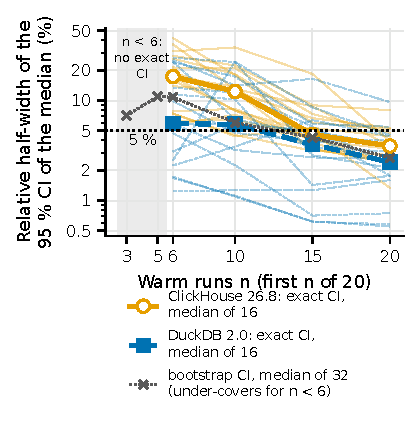
\includegraphics[width=\textwidth]{../figures/F5_repetitions.pdf}
\caption{Relative half-width of the 95\,\% CI of the median when only the first $n$ warm runs are used (thin lines: each engine, SF and query; thick lines: median per engine).}
\label{fig:reps}
\end{minipage}\hfill
\begin{minipage}[b]{0.52\textwidth}\centering
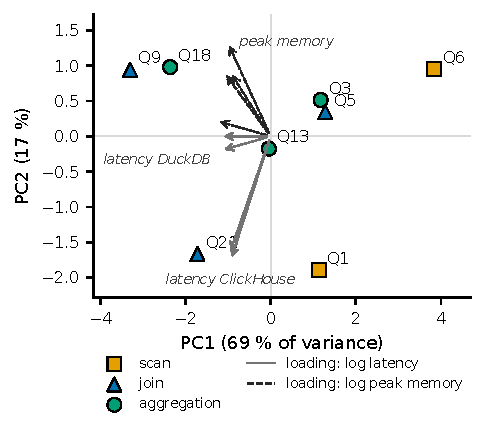
\includegraphics[width=\textwidth]{../figures/F6_pca.pdf}
\caption{PCA biplot of the eight queries; arrows show the loadings of the eight columns.}
\label{fig:pca}
\end{minipage}
\end{figure}

\section{Data needed for the full experiment}
\label{sec:needs}

Table~\ref{tab:needs} compares what the pilot collected with what we now think the full study needs, and why.

\begin{table}[!ht]
\centering\footnotesize
\caption{Data collection in the pilot and in the full study.}
\label{tab:needs}
\begin{tabularx}{\textwidth}{@{}>{\raggedright\arraybackslash}p{2.5cm}>{\raggedright\arraybackslash}p{1.9cm}>{\raggedright\arraybackslash}p{2.6cm}L@{}}
\toprule
Item & Pilot & Full study & Reason (from this pilot) \\
\midrule
Warm runs per combination & 20 & at least 20, more where needed & 20 runs gave a CI half-width below 5\,\% for \V{headline.order_share_below_5pct_n20_pct}\,\% of the combinations; 10 runs only for \V{headline.order_share_below_5pct_n10_pct}\,\% \\
Cold runs per combination & 1 & 8 (at least 6) & one run gives no CI; an exact 95\,\% CI of a median needs at least 6 runs \\
Loads per engine and SF & 3 & at least 5 & the research plan's minimum for a significant Mann--Whitney test after Holm correction \\
Scale factors & 1, 10 & 1, 3, 10 & two points always fit the scaling model; a third point gives a residual to test it \\
Memory pressure & none & a larger SF or a smaller budget & the highest peak was \V{headline.peak_max_gib}\,GiB, so spilling was never exercised \\
Concurrency & one query at a time & also two and four clients & ``who queries the data'' was the deciding factor in our qualitative exercise \\
Configuration & defaults & plus one \CH\ variant & \texttt{Float64} instead of \texttt{Decimal} or stronger compression may change RQ1 and RQ2 \\
Machine & laptop, Linux VM & dedicated Linux machine & no hidden macOS page cache; as in the research plan \\
\bottomrule
\end{tabularx}
\end{table}

\section{Discussion (e)}

\textbf{Did the results match our expectations?} Partly.
Skewed latency, slow cold runs and linear scaling all appeared, and \DK\ loaded faster and used less memory, as expected.
The main surprise is RQ1: we expected \CH\ to be faster on join and aggregation queries, but \DK\ was faster in \V{headline.n_duck_faster} of \V{headline.n_comparisons} comparisons, and \CH's tables were also larger on disk.
Warm runs were also noisier than we assumed.

\textbf{Which data were most useful?} The warm runs answered RQ1, the idle and peak container memory explained most of RQ2 (much of \CH's extra memory is its idle footprint), and the load times decided RQ3.

\textbf{Would more data help?} Yes, but of specific kinds (Section~\ref{sec:needs}): more cold runs and loads to make those comparisons testable, a third scale factor to test the scaling model, conditions that cause spilling, and concurrent queries.
More warm runs of the same kind would add little, except for the few noisy combinations.

\textbf{How general and accurate are the results?} The numbers are accurate for this set-up (every result was verified, the memory sampling agrees with the kernel's exact high-water mark, and most CIs are narrow), but they are not general.
We used one laptop with a Linux virtual machine under macOS (whose own page cache we could not empty), one run order, two SFs and default settings with four threads and \texttt{Decimal} columns, which may keep \CH\ far from its best.
The engines' own memory numbers also measure different things.
The pilot therefore shows which data the full study needs; it does not yet show which engine is better in general.

\section{Reproducibility}

All scripts, configuration, query texts, raw CSV files and this report are in our repository; \texttt{make all} rebuilds everything from data generation to this PDF, and a script checks that every number in the report comes from \texttt{results/stats/*.csv}.

\textbf{Use of AI tools.} An AI assistant (Claude, Anthropic) wrote most of the measurement and analysis scripts and drafted this report under our direction.
We reviewed the code, the data and the text, and we take responsibility for them.

\begin{thebibliography}{9}
\footnotesize\setlength{\itemsep}{0pt}\setlength{\parsep}{0pt}
\bibitem{tpch} Transaction Processing Performance Council, \emph{TPC Benchmark H Standard Specification}, Revision 3.0.1. [Online]. Available: https://www.tpc.org/tpch/
\bibitem{hoefler} T. Hoefler and R. Belli, ``Scientific benchmarking of parallel computing systems: Twelve ways to tell the masses when reporting performance results,'' in \emph{Proc. SC '15}, ACM, 2015, pp. 73:1--73:12. doi: 10.1145/2807591.2807644
\bibitem{leboudec} J.-Y. Le Boudec, \emph{Performance Evaluation of Computer and Communication Systems}. Lausanne: EPFL Press, 2010.
\bibitem{romano} J. Romano, J. D. Kromrey, J. Coraggio, and J. Skowronek, ``Appropriate statistics for ordinal level data: Should we really be using t-test and Cohen's d for evaluating group differences on the NSSE and other surveys?'' in \emph{Annual Meeting of the Florida Association of Institutional Research}, 2006.
\end{thebibliography}

\end{document}
